\subsection{Konfigurasi \textit{Deployment} Kluster Sistem Tiket}

\subsubsection{Sistem Pengawasan}

\begin{figure}[htbp]
    \centering
    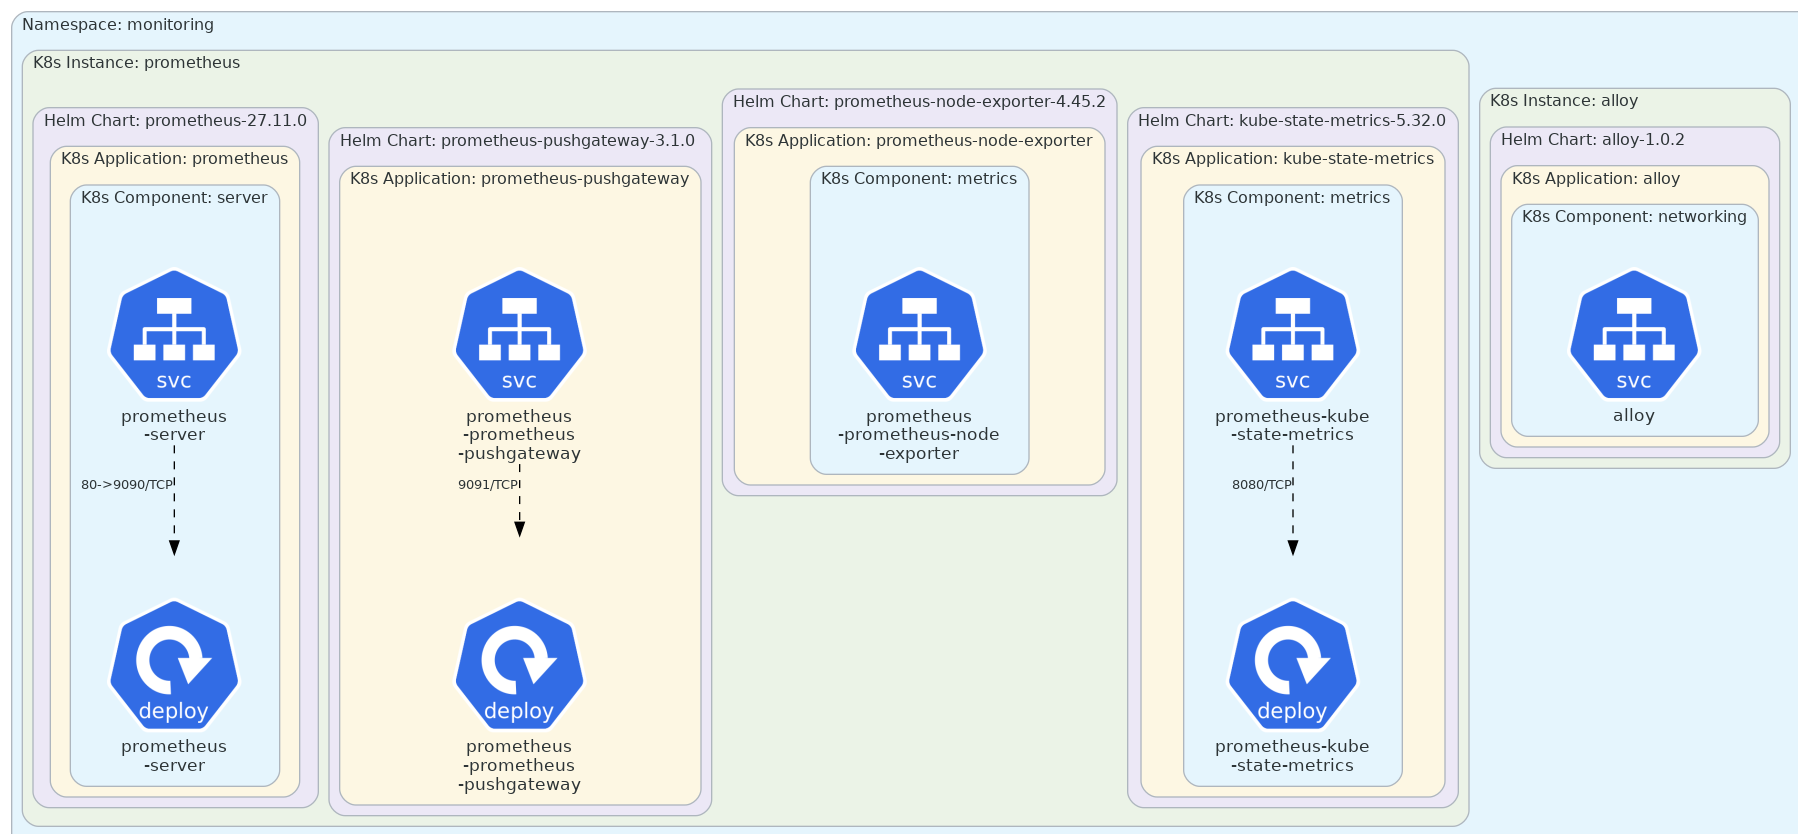
\includegraphics[width=1\textwidth]{resources/chapter-4/monitoring-1.png}
    \caption{\textit{Deployment} Sistem Pengawasan (Bagian 1)}
    \label{fig:deployment-monitoring-1}
\end{figure}

Sebagaimana dibahas pada bagian sebelumnya, komponen utama dari sistem pengawasan ini terdiri atas Grafana Alloy, Grafana Loki, Grafana Dashboard, dan Prometheus. Meskipun begitu, terdapat beberapa instans tambahan yang merupakan pengaturan bawaan dari Helm Chart yang digunakan.

\begin{figure}[htbp]
    \centering
    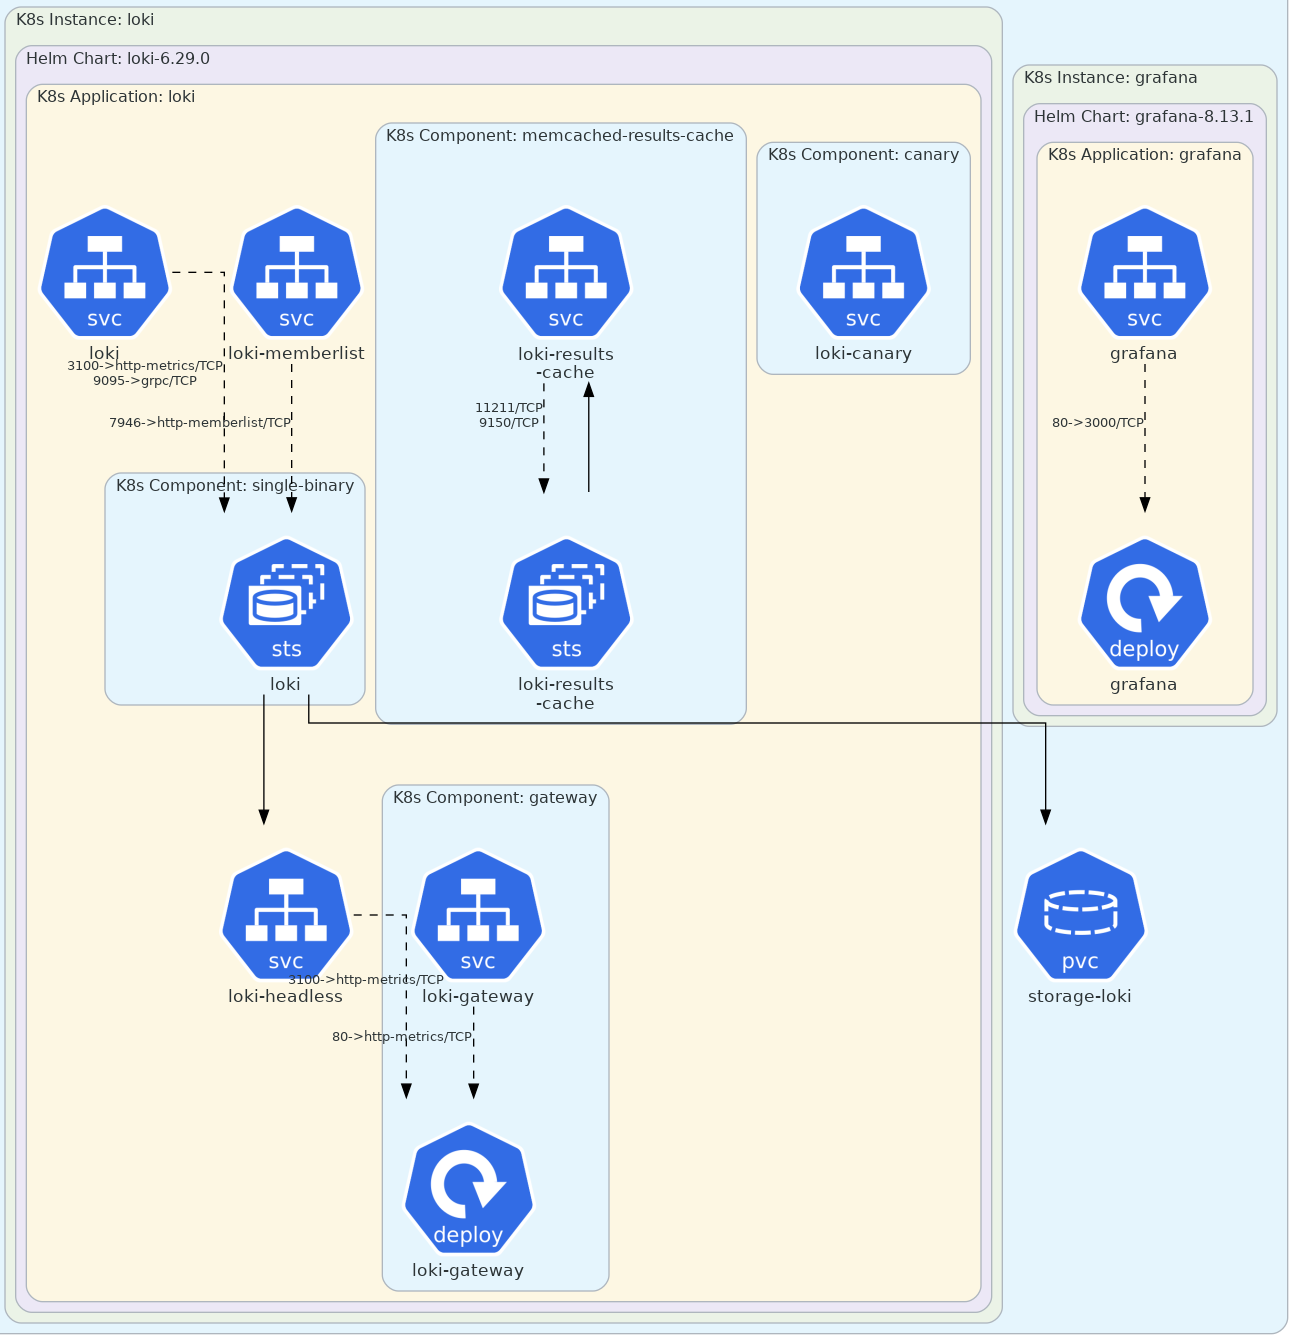
\includegraphics[width=1\textwidth]{resources/chapter-4/monitoring-2.png}
    \caption{\textit{Deployment} Sistem Pengawasan (Bagian 2)}
    \label{fig:deployment-monitoring-2}
\end{figure}

\pagebreak

\subsubsection{Nginx Ingress Controller}

\begin{figure}[htbp]
    \centering
    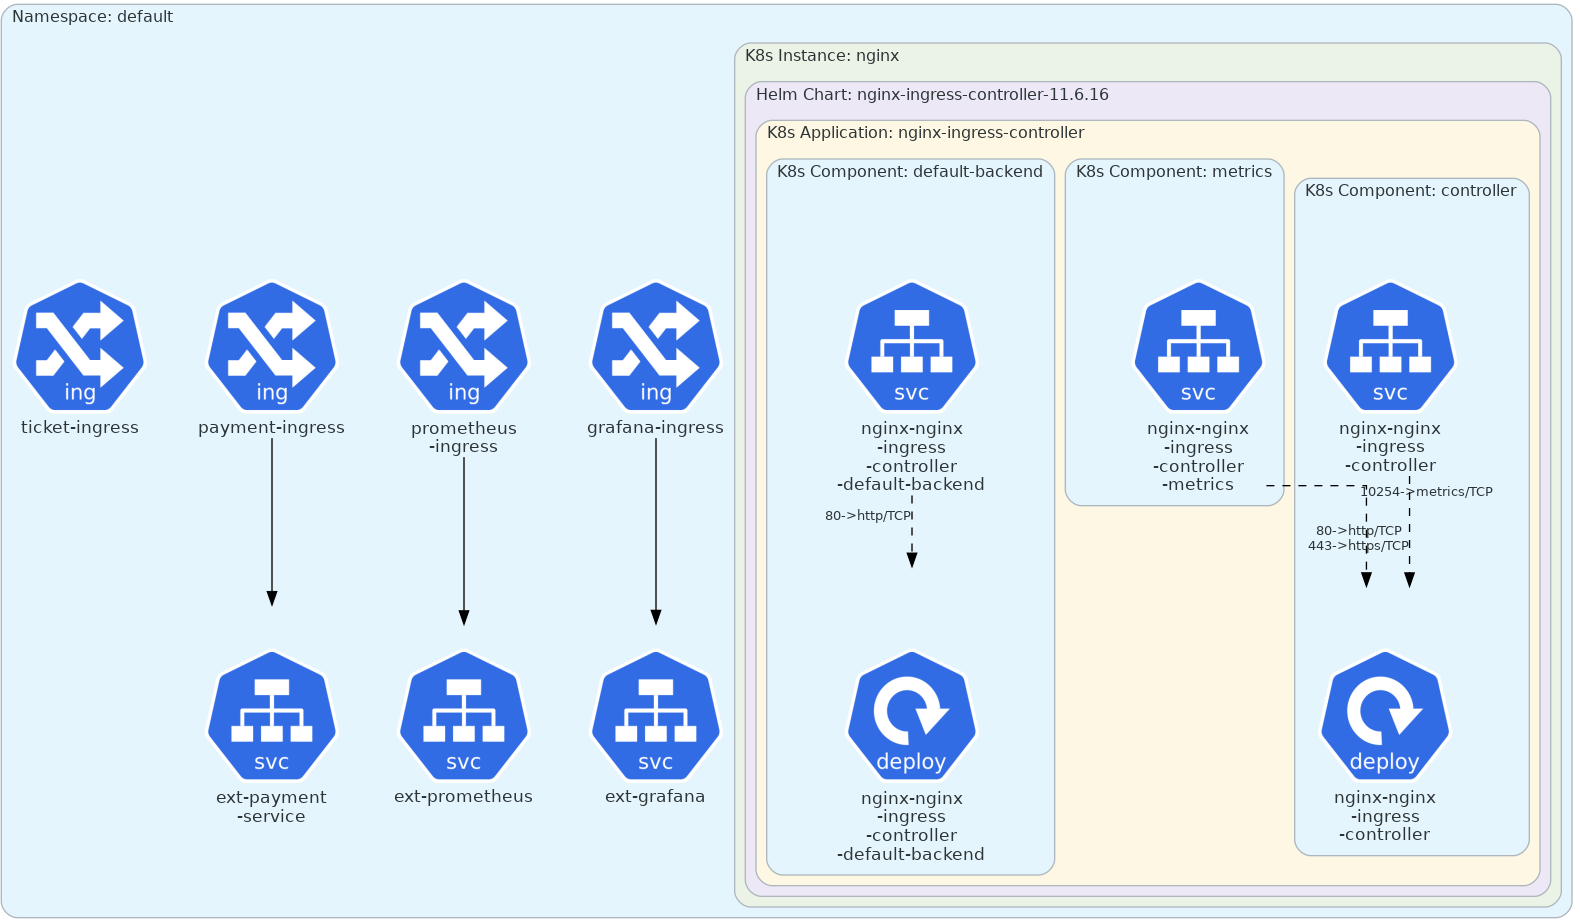
\includegraphics[width=1\textwidth]{resources/chapter-4/nginx-2.png}
    \caption{\textit{Deployment} Nginx Ingress (Bagian 1)}
    \label{fig:deployment-nginx-1}
\end{figure}

Sistem ini terdiri atas cert-manager untuk menangani sertifikat SSL domain secara otomatis, layanan Nginx Ingress Controller, serta beberapa ingress yang mengekspos layanan internal kubernetes ke dunia luar. Pada kluster ini terdapat empat \textit{service} yang diekspos, yaitu layanan tiket, layanan pembayaran, dasbor prometheus, dan dasbor Grafana.

\begin{figure}[htbp]
    \centering
    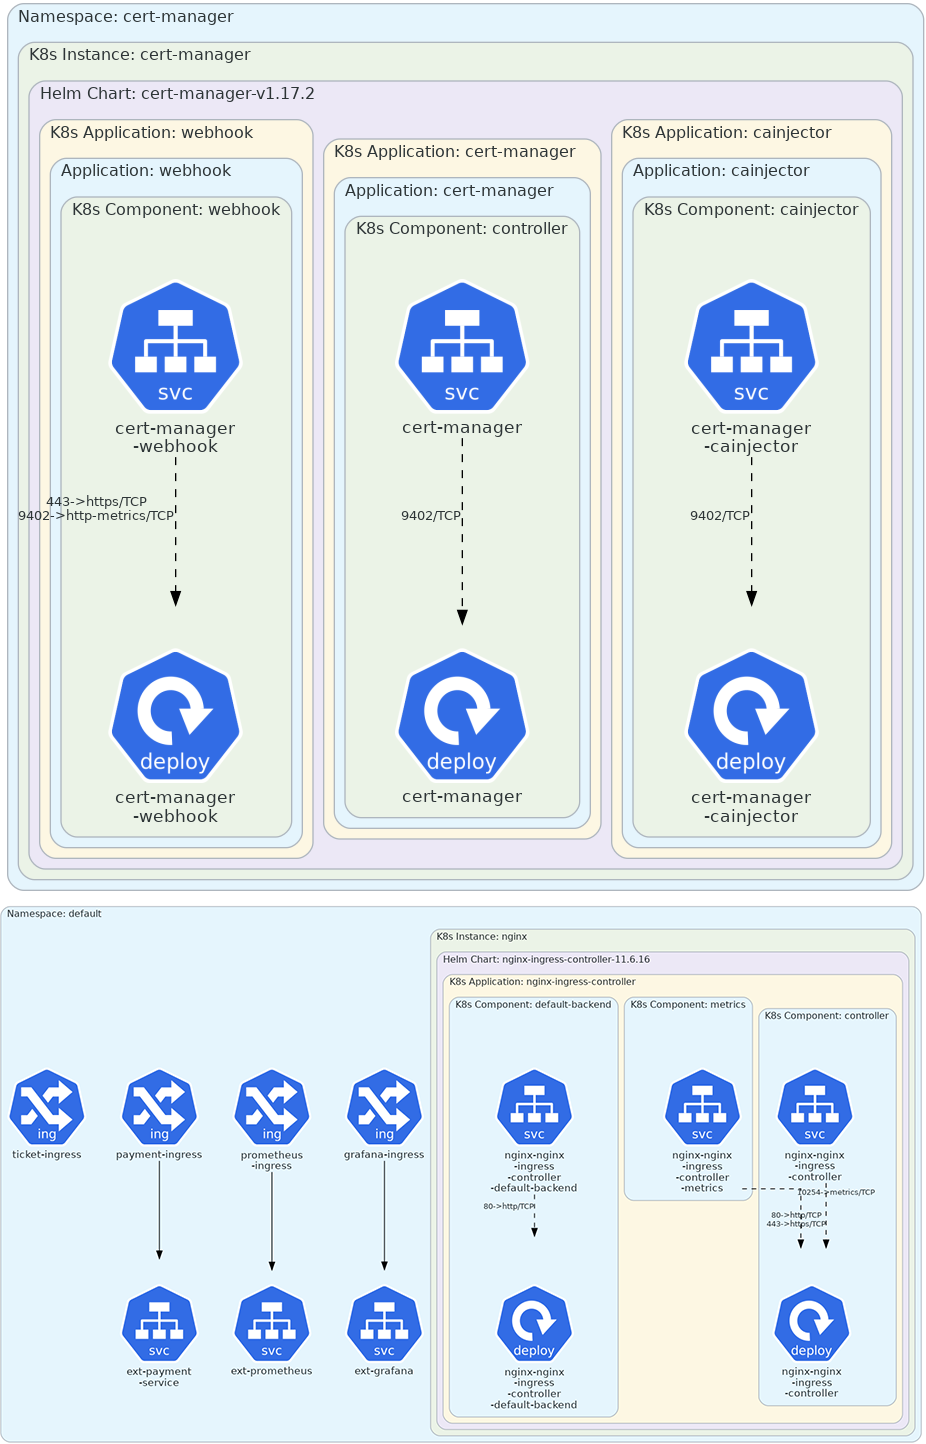
\includegraphics[width=1\textwidth]{resources/chapter-4/nginx-1.png}
    \caption{\textit{Deployment} Nginx Ingress (Bagian 2)}
    \label{fig:deployment-nginx-2}
\end{figure}

\pagebreak

\subsubsection{Layanan Pembayaran}

\begin{figure}[htbp]
    \centering
    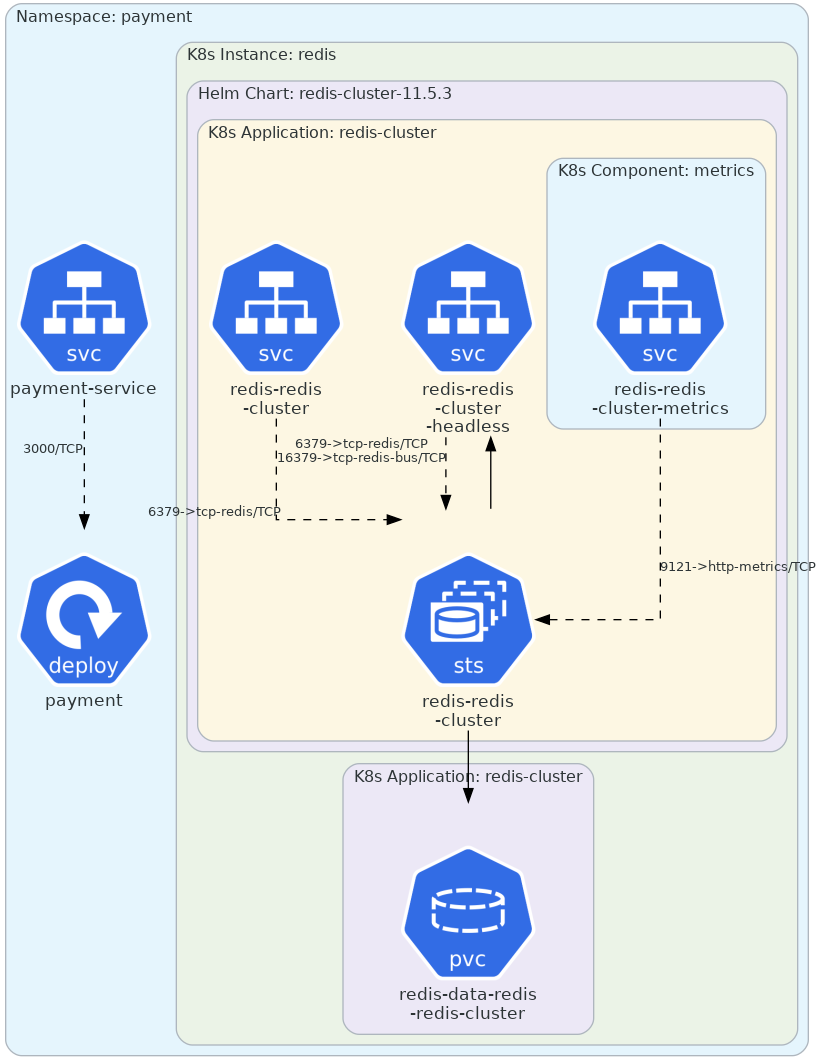
\includegraphics[width=0.8\textwidth]{resources/chapter-4/payment.png}
    \caption{\textit{Deployment} Layanan Pembayaran}
    \label{fig:deployment-payment}
\end{figure}

Layanan pembayaran secara umum terdiri atas Payment Deployment, Payment Service, dan kluster Redis. Deployment Payment terdiri atas dua kontainer, yaitu Payment Server dan Payment Notifier. Layanan ini digabung dengan kluster sistem tiket untuk mempermudah \textit{deployment}, pengujian, dan memastikan tidak ada masalah jaringan yang terjadi.

\pagebreak

\subsubsection{Layanan Tiket tanpa Pengendalian Aliran}

\begin{figure}[htbp]
    \centering
    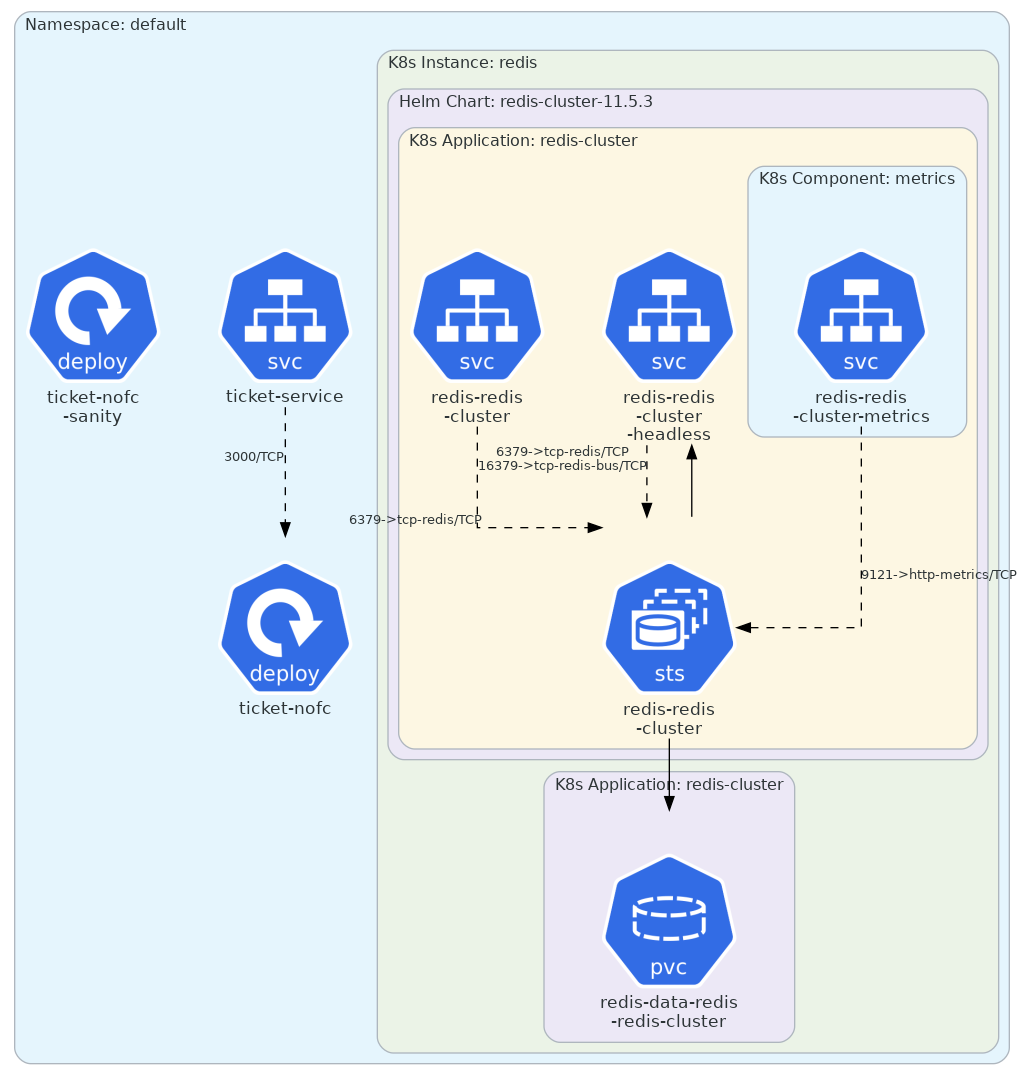
\includegraphics[width=1\textwidth]{resources/chapter-4/ticket-nofc.png}
    \caption{\textit{Deployment} Layanan Ticket tanpa Pengendalian Aliran}
    \label{fig:deployment-ticket-nofc}
\end{figure}

Layanan tiket tanpa pengendalian aliran terdiri atas Ticket Server Deployment, kluster redis, dan Sanity Check Deployment. Sistem ini juga terhubung dengan salah satu kluster basis data relasional yang ada melalui pooler PGCat.

\pagebreak

\subsubsection{Layanan Tiket varian dengan Pengendalian Aliran}

\begin{figure}[htbp]
    \centering
    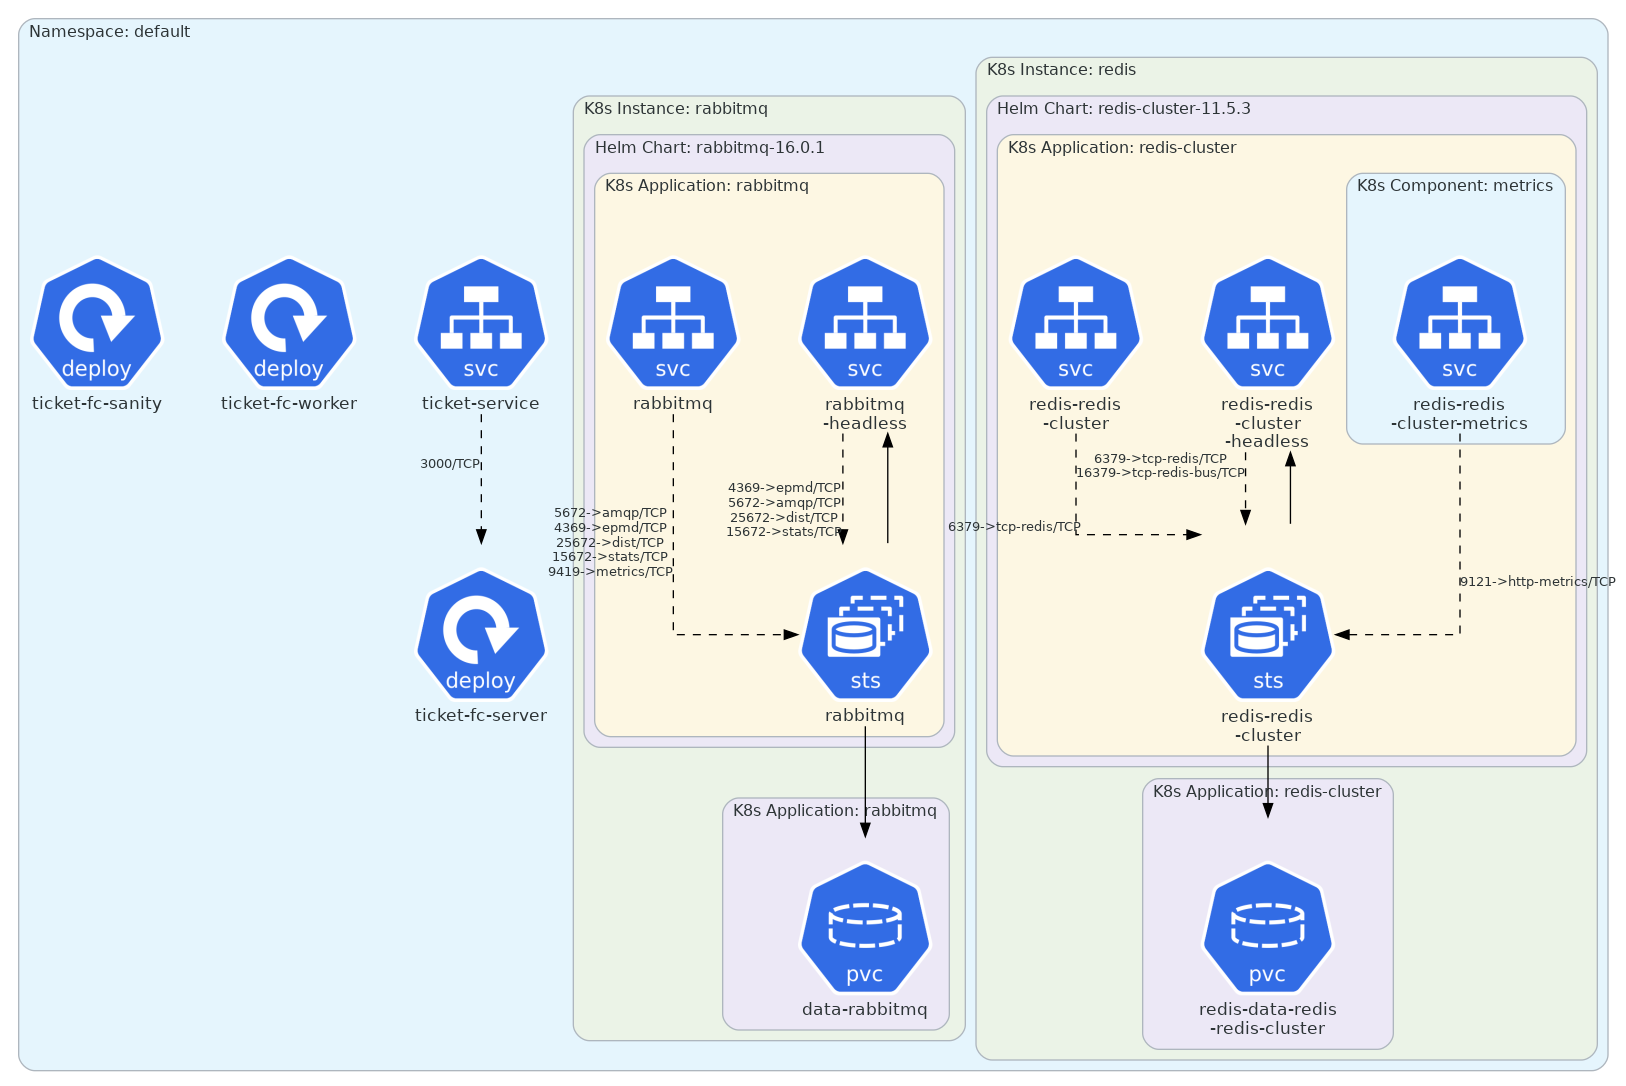
\includegraphics[width=1\textwidth]{resources/chapter-4/ticket-fc.png}
    \caption{Deployment Layanan Ticket dengan Pengendalian Aliran}
    \label{fig:deployment-ticket-fc}
\end{figure}

Layanan tiket dengan pengendalian aliran terdiri atas Ticket Server Deployment, Ticket Worker Deployment, kluster redis, RabbitMQ, dan Sanity Check Deployment. Sistem ini juga terhubung dengan salah satu kluster basis data relasional yang ada melalui pooler PGCat.

\pagebreak

\subsubsection{Kluster PostgreSQL}

\begin{figure}[htbp]
    \centering
    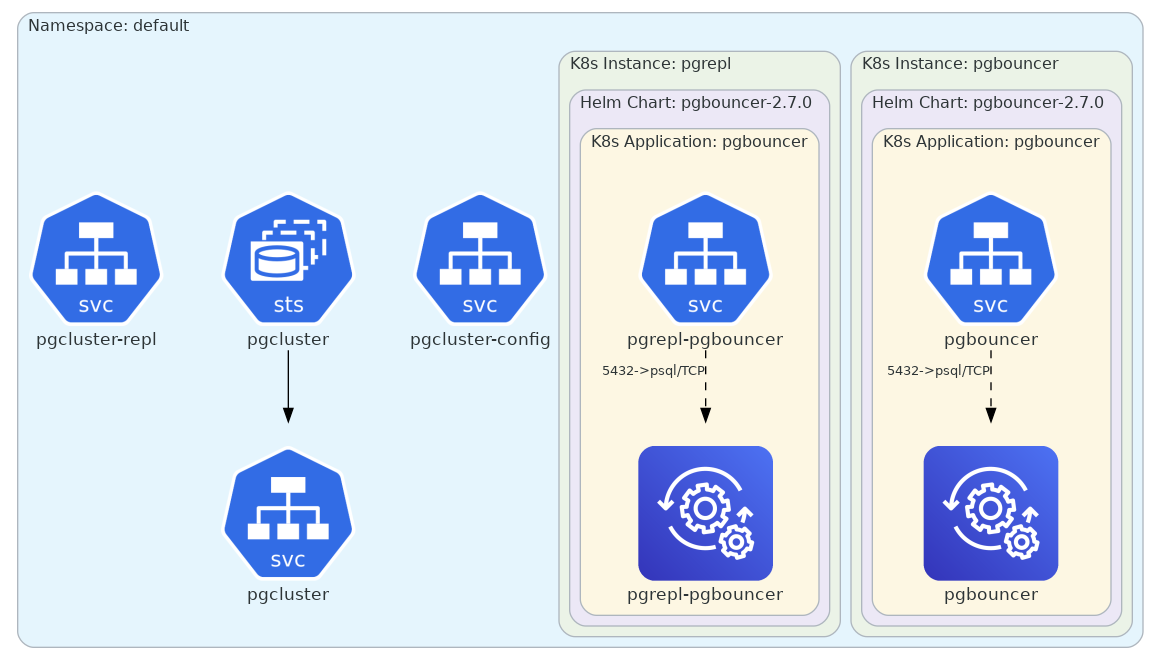
\includegraphics[width=1\textwidth]{resources/chapter-4/postgres.png}
    \caption{Deployment kluster PostgreSQL}
    \label{fig:deployment-postgres}
\end{figure}

Kluster PostgreSQL terdiri atas PostgreSQL Stateful Set yang akan terdiri atas satu \textit{primary} dan satu replika. Selain itu, terdapat PGCat yang bertindak sebagai pooler dan \textit{load balancer} pada level kueri. PGCat akan membaca kueri dan meneruskan query kepada \textit{primary} atau replika berdasarkan jenis kueri dan beban setiap instans.

\pagebreak

\subsubsection{Kluster CitusData}

\begin{figure}[htbp]
    \centering
    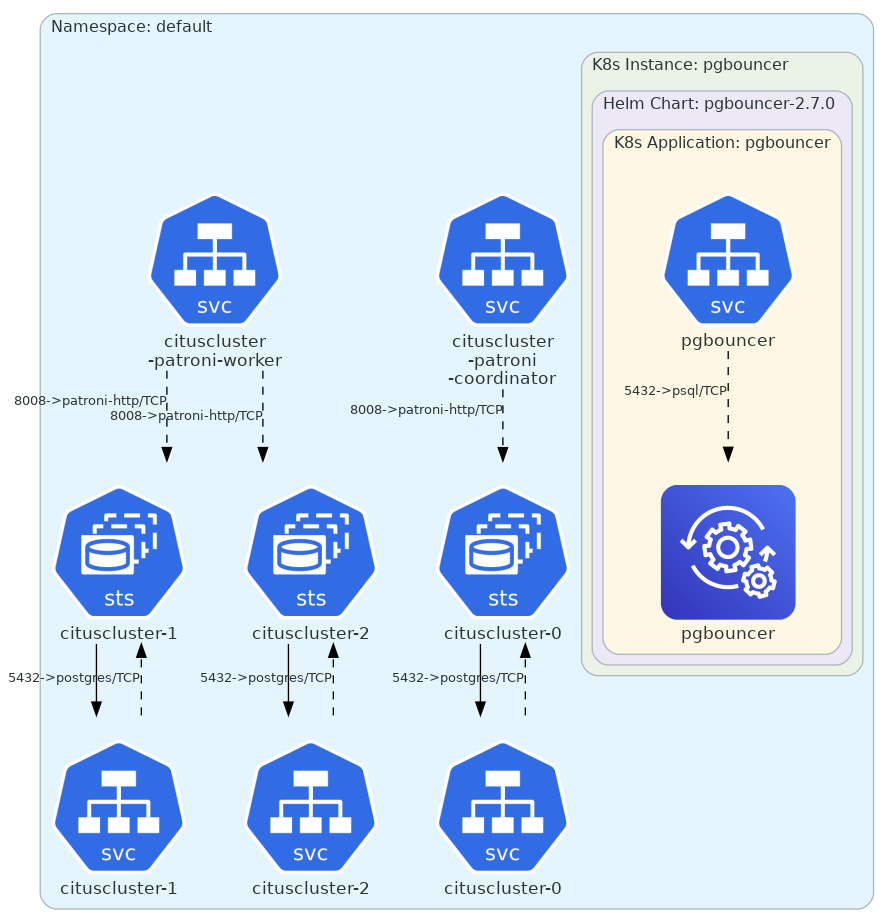
\includegraphics[width=1\textwidth]{resources/chapter-4/citusdata.png}
    \caption{Deployment kluster CitusData}
    \label{fig:deployment-citusdata}
\end{figure}

Kluster CitusData terdiri atas tiga CitusCluster Stateful Set. Kluster pertama merupakan koordinator dan sisanya merupakan pekerja. Terdapat PGCat yang terhubung dengan koordinator. Sistem tiket terhubung langsung dengan PGCat. Koneksi dengan pekerja dilakukan melalui koordinator.

\pagebreak

\subsubsection{Kluster YugabyteDB}

\begin{figure}[htbp]
    \centering
    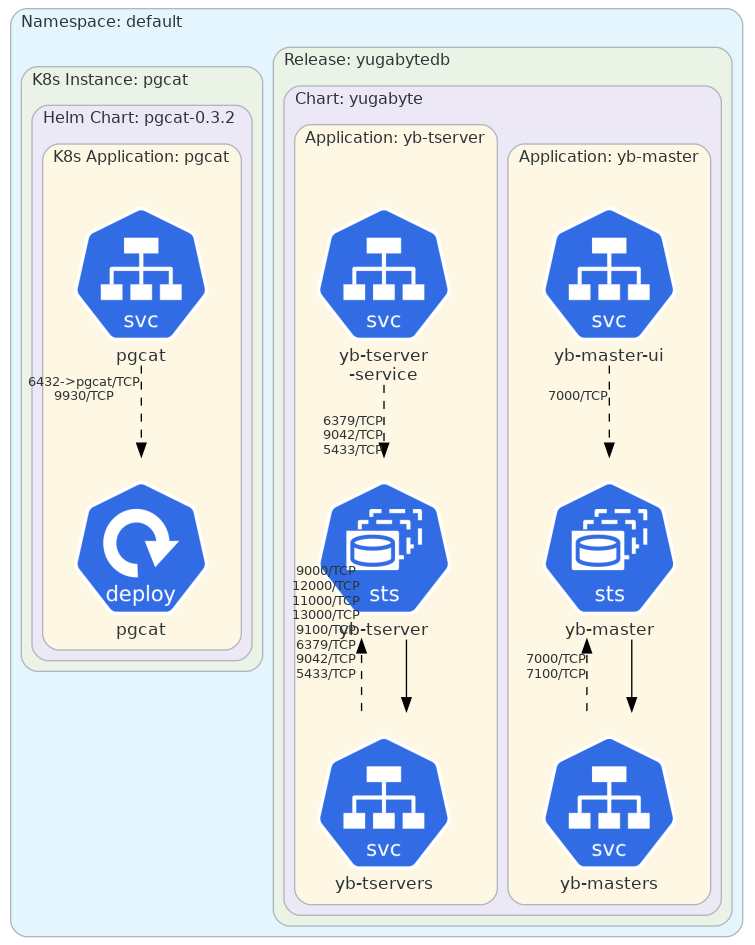
\includegraphics[width=1\textwidth]{resources/chapter-4/yugabyte.png}
    \caption{Deployment kluster YugabyteDB}
    \label{fig:deployment-yugabyte}
\end{figure}

Kluster YugabyteDB terdiri atas YB-Master Stateful Set, YB-TServer Stateful Set, dan PGCat. PGCat terhubung dengan semua instans YB-TServer. Sistem tiket terhubung langsung dengan PGCat. Proses \textit{load balancing} koneksi dengan YB-TServer ditangani oleh PGCat.

\pagebreak

\subsection{Konfigurasi \textit{Deployment} Kluster Agen Penguji}

\subsubsection{Sistem Pengawasan}

\begin{figure}[htbp]
    \centering
    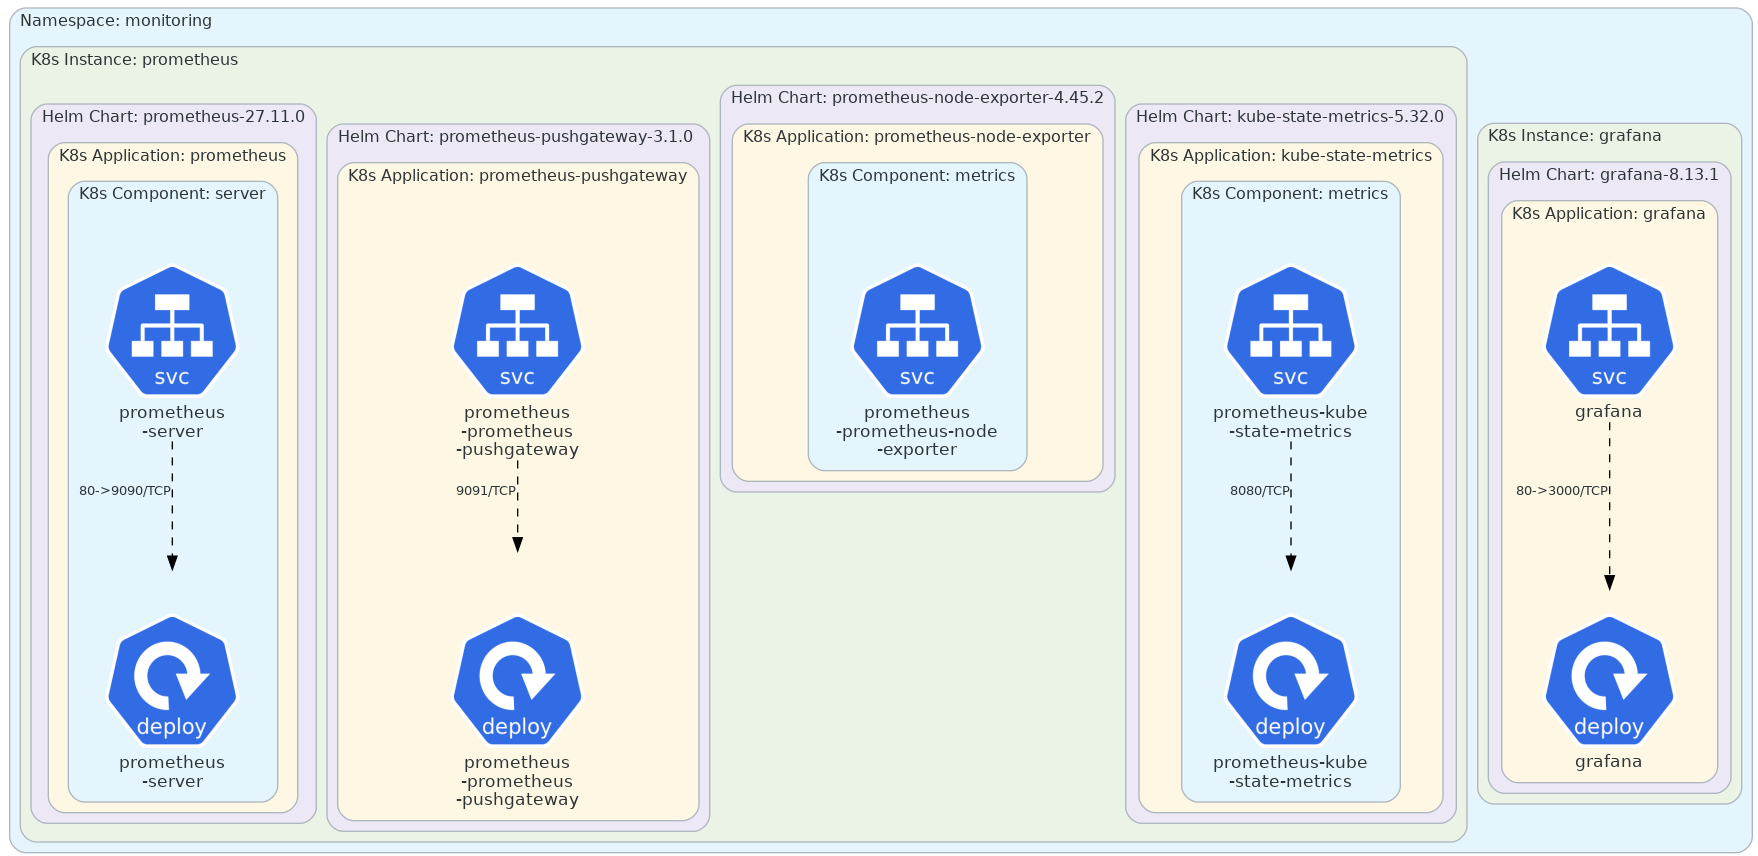
\includegraphics[width=1\textwidth]{resources/chapter-4/agent-monitoring.png}
    \caption{\textit{Deployment} Sistem Monitoring}
    \label{fig:deployment-monitoring-agent}
\end{figure}

Sistem pengawasan pada agen penguji lebih sederhana dengan komponen pengawasan hanya terdiri atas Grafana Dashboard dan Prometheus. Grafana Alloy dan Loki tidak digunakan karena \textit{log} yang relevan hanya berasal dari eksekusi K6 yang isinya dapat ditampilkan dengan perintah tertentu. Selain itu, hal ini dilakukan untuk mengurangi penggunaan sumber daya yang tidak perlu, sehingga besarnya sumber daya yang dapat digunakan untuk K6 menjadi lebih banyak.

\pagebreak

\subsubsection{Nginx Ingress Controller}

\begin{figure}[htbp]
    \centering
    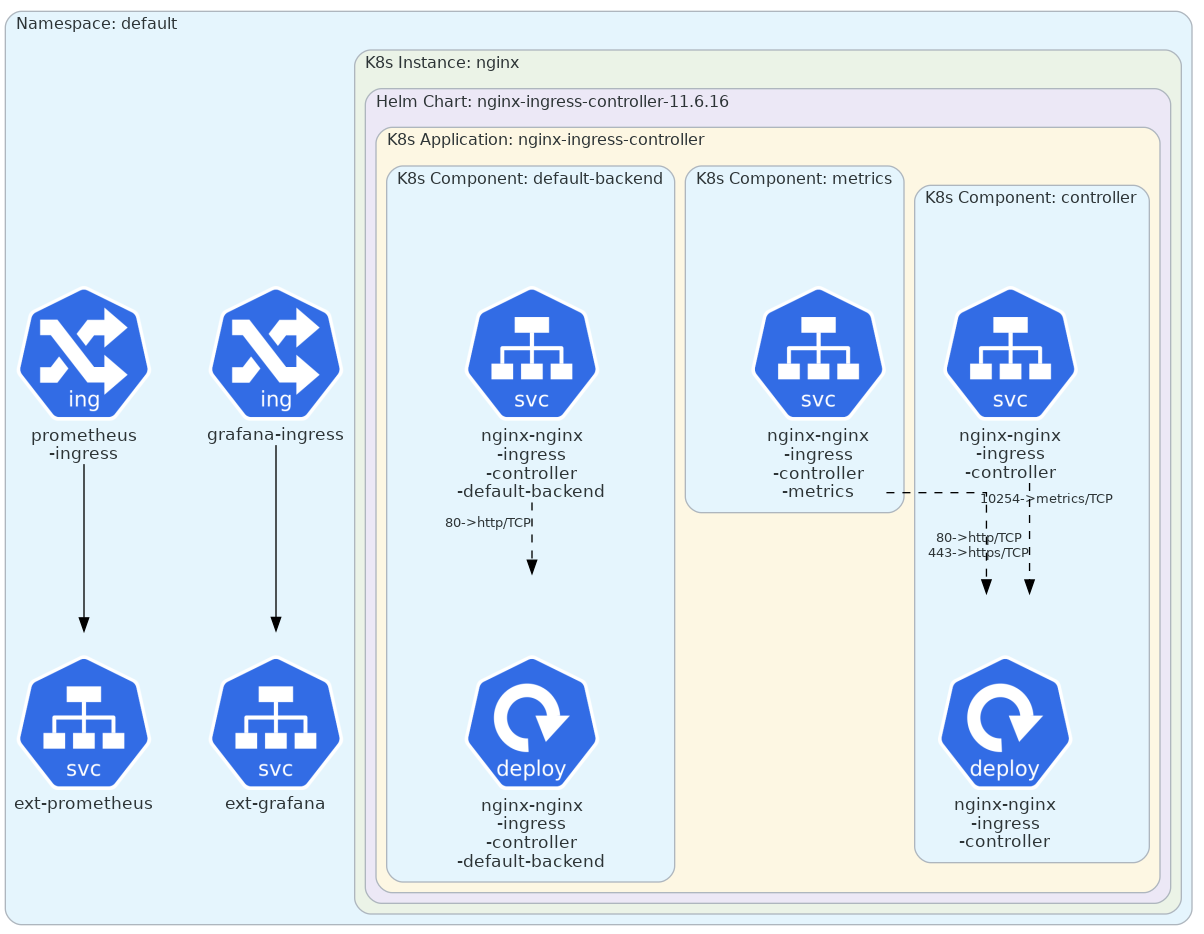
\includegraphics[width=1\textwidth]{resources/chapter-4/agent-nginx-1.png}
    \caption{Deployment Nginx Ingress}
    \label{fig:deployment-nginx-agent-1}
\end{figure}

Sistem ini terdiri atas cert-manager untuk menangani sertifikat SSL domain secara otomatis, layanan Nginx Ingress Controller, serta beberapa ingress yang mengekspos layanan internal kubernetes ke dunia luar. Pada kluster ini terdapat dua \textit{service} yang diekspos, yaitu dasbor prometheus dan dasbor Grafana. Konfigurasi cert-manager kluster penguji sama dengan konfigurasi cert-manager kluster sistem tiket sebagaimana ditunjukkan pada gambar \ref{fig:deployment-nginx-1}.

\pagebreak

\subsubsection{K6 Operator}

\begin{figure}[htbp]
    \centering
    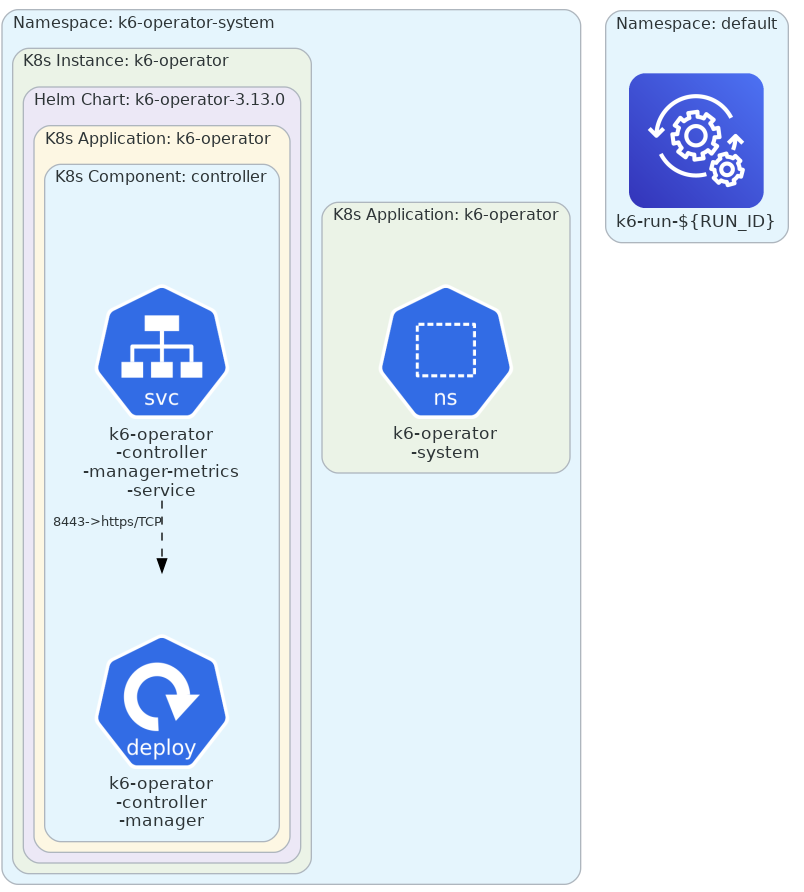
\includegraphics[width=1\textwidth]{resources/chapter-4/k6-operator.png}
    \caption{Deployment K6 Operator}
    \label{fig:deployment-k6-operator}
\end{figure}

K6 Operator merupakan komponen utama kluster penguji. Komponen ini mengatur inisiasi dan \textit{runtime} kode pengujian k6. Saat pengujian dijalankan, Grafana Operator akan menginisiasi instans K6 sebanyak 12 buah. Instans ini akan didistribusikan pada kluster.

\pagebreak